\documentclass{beamer}
\usetheme{UCLA}

\usepackage[utf8]{inputenc}
\usepackage[T1]{fontenc}

%% Fuente
\usepackage{helvet}

\title{Implementación de un Modelo Afectivo para la Arquitectura Multiagente para Sistemas Auto-Organizados y Emergentes (MASOES)}
\subtitle{Maestría en Ciencias de la Computación, Mención Inteligencia Artificial}
\author{Ing. Saúl Piña}
\date{Octubre 25, 2017}
\institute{\url{sauljabin@gmail.com}}

\begin{document}

\begin{frame}[plain,t]
\titlepage
\end{frame}

\begin{frame}
\frametitle{Agenda}
\begin{itemize}
\item Introducción
\item Objetivo General
\item MASOES
\item Modelo Afectivo de MASOES
\item Propuesta
\item Herramienta Computacional Desarrollada
\item Casos de Estudio
\item Demostración
\item Conclusión
\item Preguntas
\end{itemize}
\end{frame}

\section{Introducción}

\begin{frame}
\frametitle{Introducción}

\end{frame}

\begin{frame}
\frametitle{Computación Emocional}

\end{frame}

\begin{frame}
\frametitle{Objetivo General}
\huge
Implementar el modelo afectivo de MASOES en un sistema multiagente
\end{frame}

\section{MASOES}

\begin{frame}
\frametitle{MASOES}

\end{frame}

\begin{frame}
\frametitle{MASOES}
La arquitectura multiagente para sistemas emergentes y auto-organizados llamada
MASOES (Multiagent Architecture for Self-Organizing and Emergent Systems, en inglés),
es una herramienta para el diseño no
formal de sistemas, que produzcan un estado auto-organizado el cual emerja de
las interacciones locales entre los agentes y de los cambios que se dan en el
entorno. En esta arquitectura, cada agente puede cambiar su comportamiento
dinámicamente, guiado por su estado emocional, para satisfacer dinámicamente los
objetivos del sistema a través de la auto-organización de sus actividades.
\end{frame}

\begin{frame}
\frametitle{MASOES}
\framesubtitle{Modelo Afectivo de MASOES}
El modelo afectivo (o emocional) de MASOES considera un conjunto de
emociones positivas y negativas generadas desde un nivel individual o colectivo,
para de esta manera promover un comportamiento individual (Reactivo, Cognitivo)
o colectivo (Imitativo) en los agentes y así, aumentar su grado de satisfacción
y por consecuencia, el nivel de auto-organización y emergencia general en el
sistema.
\end{frame}

\begin{frame}
\frametitle{MASOES}
\framesubtitle{Modelo Afectivo de MASOES}
\begin{columns}
\column{0.5\textwidth}
Este modelo afectivo está representado por un espacio bidimensional,
donde el eje $x$ representa el nivel de \textbf{Activación} del agente en el
intervalo $[-1, 1]$, y el eje $y$ representa el nivel de \textbf{Satisfacción},
también en el intervalo $[-1, 1]$.
\column{0.5\textwidth}
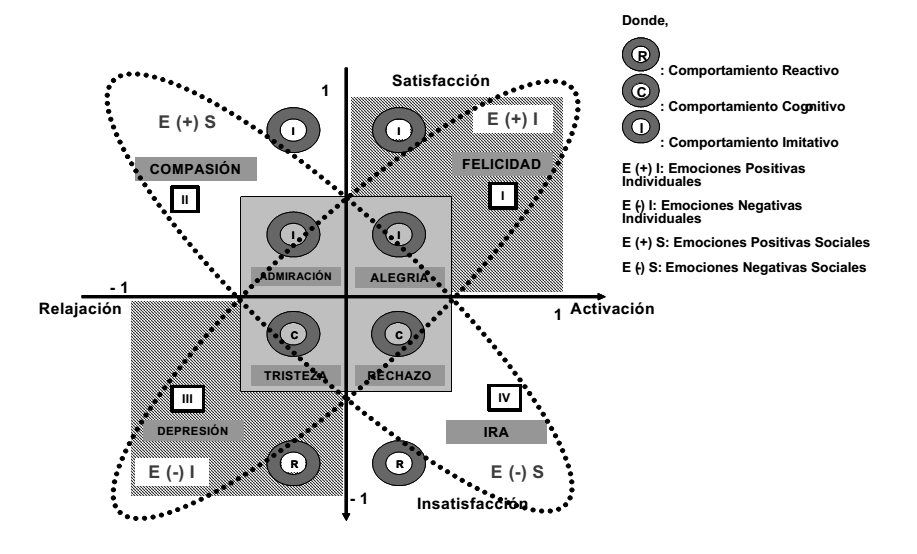
\includegraphics[width=5cm]{ilustraciones/modelo-afectivo}
\end{columns}
\end{frame}

\section{Propuesta}

\begin{frame}
\frametitle{Propuesta}
\framesubtitle{Aspectos Arquitecturales}
\begin{columns}
\column{0.5\textwidth}
\textbf{JADE}\\
\textbf{Java Agent
DEvelopment}, uno de los marcos de trabajo con paradigma de POA \textbf{Programación Orientada a Agentes}
más populares, implementado en el lenguaje de programación Java
\column{0.5\textwidth}
\textbf{FIPA}\\
\textbf{Foundation for Intelligent Physical Agents},
las cuales representan una colección de normas que tienen como objetivo promover la interoperabilidad
de agentes heterogéneos y los servicios que pueden representar
\end{columns}
\end{frame}

\begin{frame}
\frametitle{Propuesta}
\framesubtitle{Aspectos Arquitecturales}
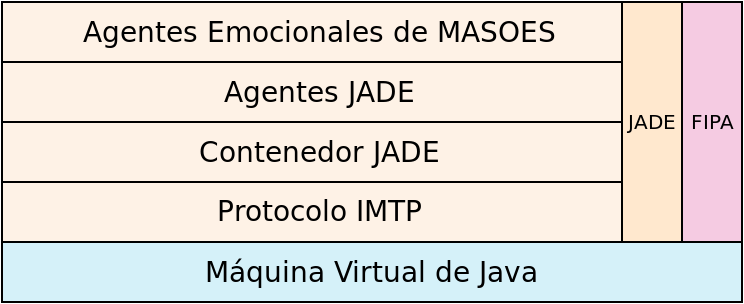
\includegraphics[width=8cm]{ilustraciones/arquitectura}
\end{frame}

\begin{frame}
\frametitle{Propuesta}
\framesubtitle{Comunicación Entre Agentes}
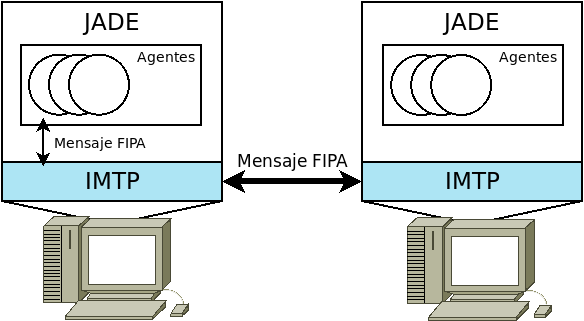
\includegraphics[width=8cm]{ilustraciones/comunicacion-entre-hosts}
\end{frame}

\begin{frame}
\frametitle{Aspectos Propuestos a Nivel Individual}

\end{frame}

\begin{frame}
\frametitle{Aspectos Nivel Colectivo}

\end{frame}

\begin{frame}
\frametitle{Herramienta Computacional}

\end{frame}

\section{Casos de Estudio}
\begin{frame}
\frametitle{Casos de Estudio}

\end{frame}

\DoBlueBackgroundTitle{Demostración}

\section{Conclusión}
\begin{frame}
\frametitle{Aportes}

\end{frame}

\begin{frame}
\frametitle{Conclusión}

\end{frame}

\DoBlueBackgroundTitle{Preguntas}

\ThankYouFrame

\end{document}
